\documentclass{anstrans}
%%%%%%%%%%%%%%%%%%%%%%%%%%%%%%%%%%%
\title{Dynamic Resource Exchange Performance in Cyclus}
\author{Matthew J.~Gidden, Paul P. H.~Wilson}

\institute{
University of Wisconsin, Madison WI
}

\email{gidden@wisc.edu}

%%%% packages and definitions (optional)
\usepackage{graphicx} % allows inclusion of graphics
\usepackage{booktabs} % nice rules (thick lines) for tables
\usepackage{microtype} % improves typography for PDF

\usepackage{multirow} % combining rows in tables
\usepackage{tabularx} % for tables with line breaks

\newcommand{\Cyclus}{\textsc{Cyclus}}
\newcommand{\ffc}{$f_{\text{fc}}$}
\newcommand{\frx}{$f_{\text{rx}}$}
\newcommand{\floc}{$f_{\text{loc}}$}

\begin{document}

%%%%%%%%%%%%%%%%%%%%%%%%%%%%%%%%%%%%%%%%%%%%%%%%%%%%%%%%%%%%%%%%%%%%%%%%%%%%%%%%
\section{Introduction}

Nuclear fuel cycle simulation is a field which seeks to model the facilities and
material flows required to produce nuclear power. Simulations normally model a
time span of decades, or even centuries. Myriad decisions exist within a given
fuel cycle simulation, such as the deployment timing of facility types and
determining how material transfers should be executed at a given time
step. Accordingly, trade-offs exist between the features provided by a simulator
and the performance of the simulator.

The \Cyclus{} simulator \cite{cyclus2014} was designed to more easily model a
variety of fuel cycles. It uses an agent-based modeling paradigm, encapsulating
the difficulty of designing new agent archetypes. Archetypes define
parameterized agent logic and behavior and can therefore be reused within and
between simulations. The core agent-interaction model in \Cyclus{} is the
Dynamic Resource Exchange (DRE) \cite{gidden_agent-based_2013,
  gidden_agent-based_2014}. The DRE, recomputed at each time step, polls the
supply and demand of commodities in the simulation and then determines the
trades to be executed between agents. Highly dynamic, easily adjustable fuel
cycles can be modeled by coupling the DRE concept with the \Cyclus{}
Region-Institution-Facility hierarchy and archetype-prototype-agent models,
addressing many of the issues developers and users have found with previous
models. However, \Cyclus{} must both be featureful and performant. This work
provides a first-look at how the DRE supply-demand model scales with problem
size by generating and solving a large number of exchanges. Different solvers
are analyzed including a \Cyclus{}-aware greedy heuristic in addition to
COIN-OR's LP and MILP solvers \cite{coinclp, coincbc}.

%%%%%%%%%%%%%%%%%%%%%%%%%%%%%%%%%%%%%%%%%%%%%%%%%%%%%%%%%%%%%%%%%%%%%%%%%%%%%%%%
\section{Methodology}

Instances of resource exchanges are required to analyze the effects and
performance of the DRE and its solvers. In the absence of large Cyclus
simulations with interesting facility and relationship models, relevant
instances must be generated outside of Cyclus given some set of rules and
parameters. Two distinct \textit{species} of exchanges are generated, those
related to the \textit{front end} of the nuclear fuel cycle and those related to
the \textit{back end} of the nuclear fuel cycle. For each species, commodities,
reactors, and supporting facilities must be generated in addition to
exchange-related parameters, such as the trade preferences.

Three types of fuel cycles are generated: a once-through fuel cycle, labeled
OT; a plutonium-recycle fuel cycle, labeled MOX; and a plutonium and
thorium-recycle fuel cycle, labeled MOX-ThOX. As fuel cycles increase in
complexity, the number of commodities that exist increases, as shown in Table
\ref{tbl:fc_to_commods}. The commodities are referred to by abbreviation:
Uranium Oxide (UOX), Mixed Plutonium Oxide for Thermal Reactors (TMOX), Mixed
Plutonium Oxide for Fast Reactors (FMOX), Thorium Oxide for Fast Reactors
(FThOX).

\begin{table}[]
\centering
\caption{A mapping between fuel cycles to the commodities that exist in each one.}
\label{tbl:fc_to_commods}
\begin{tabular}{|c|c|}
\hline
\textbf{Fuel Cycle}            & \textbf{Commodities} \\ \hline
OT                    & UOX         \\ \hline
\multirow{3}{*}{MOX}  & UOX         \\  
                      & TMOX        \\  
                      & FMOX        \\ \hline
\multirow{4}{*}{ThOX} & UOX         \\  
                      & TMOX        \\  
                      & FMOX        \\  
                      & FThOX       \\ \hline
\end{tabular}
\end{table}

All reactors are modeled as either thermal or fast reactors. It is necessary to
estimate the amount of fuel exchanged by reactors each time step. Accordingly,
thermal reactors are simplified models of AP-1000 reactors, and fast reactors
are simplified models of BN-600 reactors. Reactors operate in a batch mode,
where each batch is approximately one quarter of the reactor core, an assumption
used by other analyses \cite{rineiski2011reactivity}. Each reactor in the
exchange is either offering or requesting a batch of fuel. Reactors may be
fueled by different fuel types, i.e., fuel commodities. A mapping of reactors to
acceptable commodities is provided in Table \ref{tbl:rx_to_commods}. Note that
there is still a preference distribution associated with each reactor-commodity
pair as well as constraint coefficient effects; therefore, while a reactor
\textit{can} consume a fuel commodity, it may do so only in the absence of any
other commodity availability. It is assumed that a reactor would rather utilize
an undesirable fuel type than realize the lost revenue from not producing power.

\begin{table}[]
\centering
\caption{A mapping between reactor types and the commodities allowed to fuel 
  each reactor type.}
\label{tbl:rx_to_commods}
\begin{tabular}{|c|c|}
\hline
\textbf{Reactor Types}            & \textbf{Fuel Commodities} \\ \hline
\multirow{3}{*}{Thermal}                    & UOX         \\ 
                      & TMOX        \\  
                      & FMOX       \\ \hline
\multirow{4}{*}{FMOX}  & UOX         \\  
                      & TMOX        \\ 
                      & FMOX        \\  
                      & FThOX        \\ \hline 
\multirow{4}{*}{FThOX} & UOX         \\  
                     & TMOX        \\ 
                      & FMOX        \\  
                      & FThOX        \\ \hline 
\end{tabular}
\end{table}

In a front-end exchange, fuel suppliers exchange material with reactors. In a
back-end exchange, reprocessing and storage facilities exchange material with
reactors. In either case, facilities that are \text{not} reactors are referred
to as \textit{support} facilities, as they support the reactors which generate
power. In the front-end exchange model, a single type of supporting facility
exists for each fuel type, e.g., an enrichment facility for UOX, a thermal
reprocessing plant for TMOX, etc. In the back-end exchange model, a similar
supporting facility assignment is used, except a storage facility type, capable
of storing any commodity is added.

For reactors and support facilities in both exchange species, exchange
constructs, such as preferences and constraint coefficients, must be
generated. Constraint coefficients are a function of resource quality, for which
a proxy must be assigned. Accordingly, each reactor is modeled using an
enrichment-level-range-to-commodity mapping. For example, LWRs requesting UOX
have an enrichment range of $[3.5, 5.5]$. The enrichment value for each reactor
is chosen from a uniform distribution in order to differentiate
reactors. Preferences in the DRE are requester-based, and are assigned
per-commodity to requesters in both exchange species. In order to differentiate
between preferences, facilities are assigned a location proxy. The location
proxy can provide additional weight to preference values.

Exchange generation is parameterized and thus depends on a parameter
vector. While each species has specific parameters, both species share some
fundamental parameters, namely: \ffc, which fuel cycle is being generated; \frx,
whether reactors are modeled using a single batch or a collection of assemblies;
and \floc, to what degree location is used in determining preference
coefficients. \ffc may take on values of OT, MOX, or THOX, as described
above. \frx may take on values of Batch or Assembly. \floc may take on values of
None, Coarse, or Fine.

%% \begin{table}[]
%% \centering
%% \caption{Parameter Description Summary for Species-Independent Parameters.}
%% \label{tbl:global_params}
%% \begin{tabularx}{\columnwidth}{|c|X|c|} % line wraps second column if too long
%% \hline
%% Parameter    & 
%% Description & 
%% Values
%% \\ \hline
%% \ffc      &
%% Which fuel cycle is being modeled &
%% OT, MOX, THOX
%% \\ \hline
%% \frx    &
%% Whether individual assemblies are modeled or whole batches are modeled &
%% Batch, Assembly  
%% \\ \hline
%% \floc     &
%% To what degree is facility location included in objective coefficients &
%% None, Coarse, Fine
%% \\ \hline
%% \end{tabularx}
%% \end{table}

Given a set of parameters, an exchange instance is generated and persisted in a
database. The generated exchange exists in the \textit{exchange layer} of the
DRE, as shown in Figure \ref{fig:dre_time}. Because the greedy heuristic is
knowledgeable of \Cyclus, it uses solution pathway $1$ shown in the figure. The
COIN solvers must have the \Cyclus{} exchange structure formulated into a
mathematical program, described previously in \cite{gidden_agent-based_2013},
and thus must take the second solver pathway, through the formulation
layer. Figure \ref{fig:dre_time} also notes the time points measured during
execution in order to compare solution times between solvers and different
exchange instances, i.e., for each solver and exchange instance, execution time
is measured as $t_f - t_i$.

\begin{figure*}
  \begin{center}
    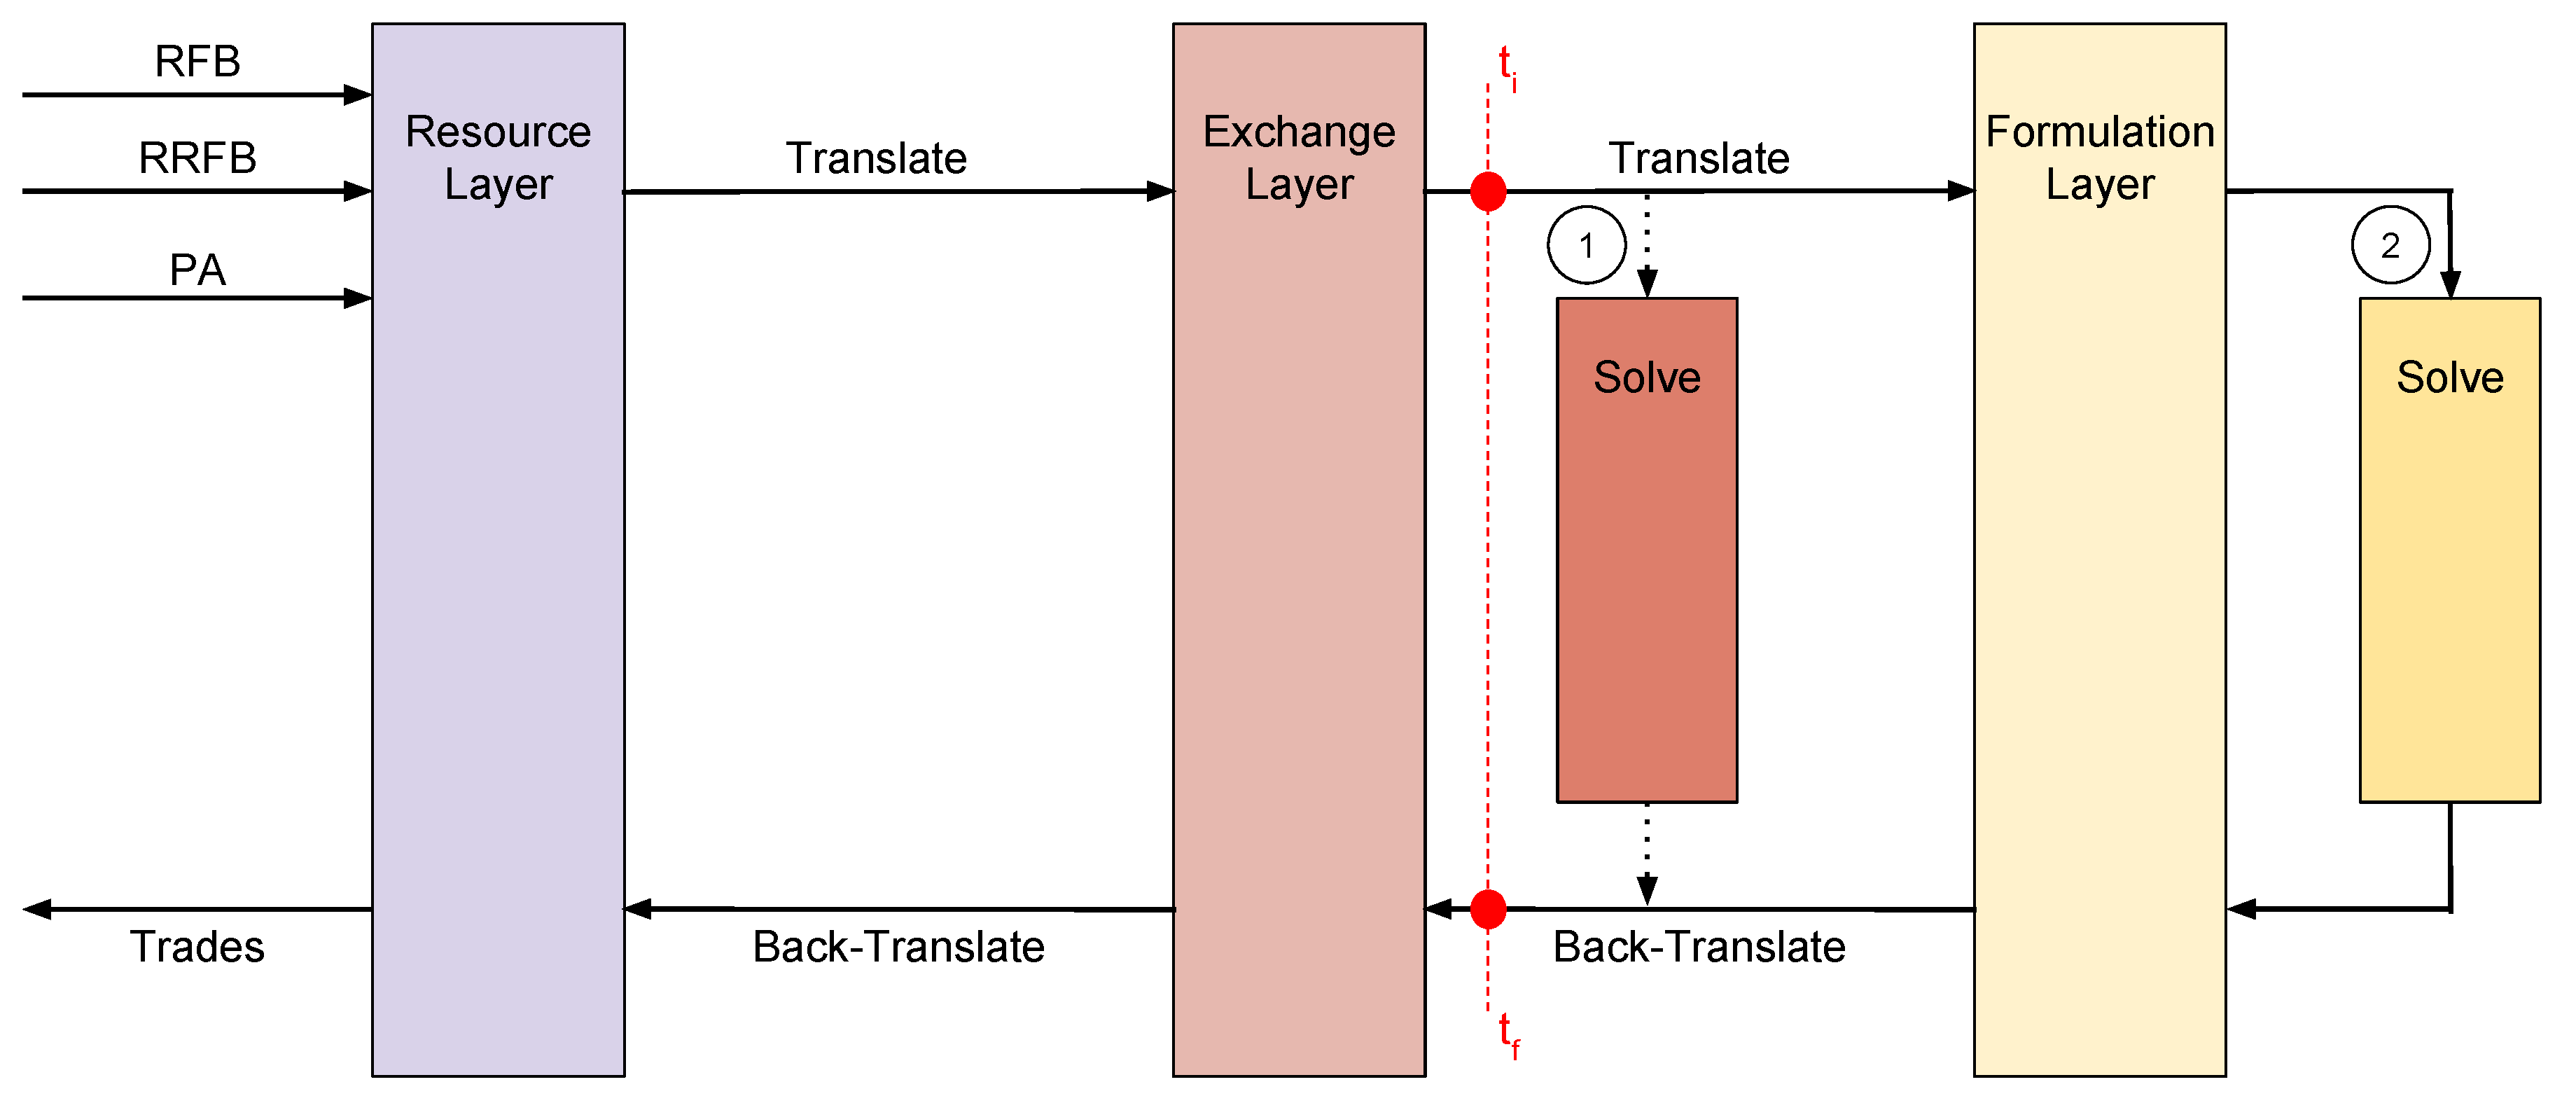
\includegraphics[width=2\columnwidth]{exchange_xlation_timing.pdf}
    \caption[]{
      \label{fig:dre_time}
      The control flow of the DRE execution and time points for comparing
      different solutions. The greedy heuristic takes the pathway labeled $1$,
      while CLP and CBC solvers take the second pathway. The DRE workflow is
      described more fully in \cite{gidden_agent-based_2013,
        gidden_agent-based_2014}. }
  \end{center}
\end{figure*}

In order to explore the large number of possible exchange instances, a
sophisticated instance generation and solving framework is needed. Accordingly,
a new software package called Cyclopts (\underline{Cycl}us
\underline{Opt}imization \underline{S}tudies) has been developed. Cyclopts
provides a general framework for sampling a parameter space, defining problem
instances for a given point in parameter space, and solving a problem instance
under a variety of conditions. Cyclopts leverages an HTCondor-aware High
Throughput Computing (HTC) framework at UW-Madison in order to efficiently run
exchange instances.

An experiment consists of a set of resource-exchange graph instances executed
with a collection of configured solvers. When a solution is found, the solution
(i.e., the flow vector), the time required to reach the solution, and the
objective value (i.e., the dot-product of cost and flow vectors) are
recorded. Six execution nodes on UW-Madison Advanced Computing Initiative (ACI)
HTCondor system form the homogeneous environment used to conduct the experiments
herein described. Each execute node is comprised of an 2.90 GHz eight-core,
sixteen-thread, Intel Xeon E5-2690 processor with 128 GB of RAM. Processor
hyper-threading was disabled for the duration of the experimental campaign to
allow comparisons between solution times.

%%%%%%%%%%%%%%%%%%%%%%%%%%%%%%%%%%%%%%%%%%%%%%%%%%%%%%%%%%%%%%%%%%%%%%%%%%%%%%%%
\section{Results and Analysis}

A scalability campaign was launched to study how the solvers perform as the size
of exchange increases. All species-specific parameters for generating an
exchange are a function of the number of reactors in the exchange, thus the
number of reactors in the system is the natural choice for a scaling
parameter. A range of $[10, 500]$ was chosen for this analysis. For each reactor
population value, exchanges were generated for all possible combinations of
fundamental parameter values ($18$ total). Each generated exchange instance was
solved with all three available solvers. Figure \ref{fig:greedy_size} provides
an example of output from the scalability campaign.

\begin{figure*}
  \begin{center}
    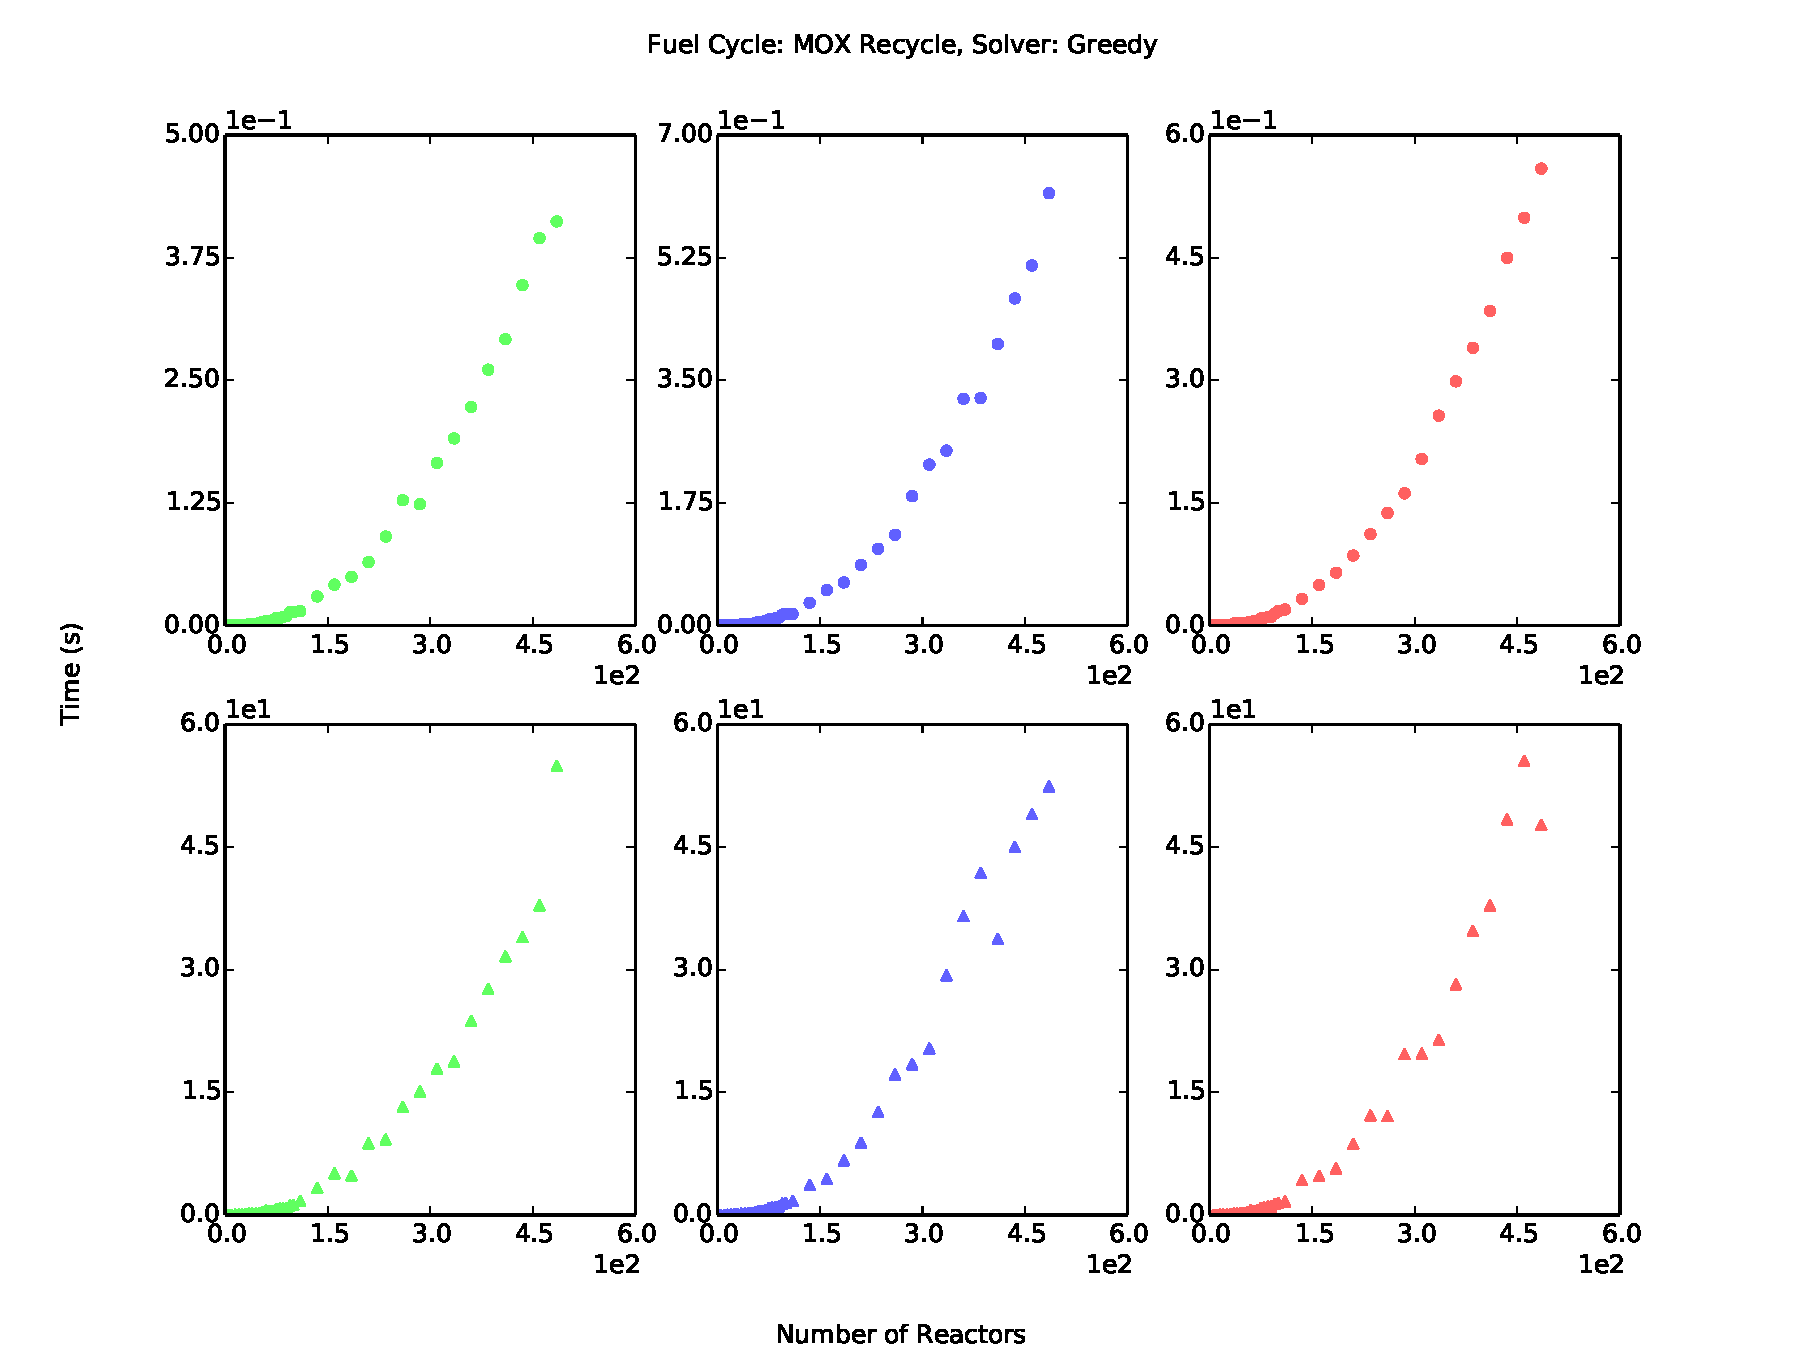
\includegraphics[width=1.5\columnwidth]{base_back_n_rxtr_time_fc1_solvergreedy.pdf}
    \caption[]{
      \label{fig:greedy_size}
      Results for the size scoping study for the greedy heuristic modeling a
      back-end MOX fuel cycle. Rows have increasing \frx values and columns have
      increasing \floc values.}
  \end{center}
\end{figure*}

Both the CLP and greedy solvers were found to scale similarly. As shown in
Figure \ref{fig:greedy_size}, polynomial scaling ($\mathcal{O}(n^2)$) in the
reactor population is observed. This is driven by the number of constraints in
the resulting formulation, rather than the number of variables, for which linear
scaling ($\mathcal{O}(n)$) was observed. Polynomial scaling of both the greedy
and CLP solvers occurs regardless of fundamental parameter or exchange
species. The CBC solver, however, performs sporadically, with many exchange
instances remaining unconverged at a $3$-hour time cap. This is not unexpected,
as solving a MILP optimally is an NP-hard problem. Most exchanges consisting of
$100$ (or less) reactors was found to converge well below the cap.

Every exchange instance depends on both objective value and constraint
coefficients, both of which are products of stochastic processes. Accordingly,
an experimental campaign was launched to study the effects of stochasticity on
the solution times and relative solution values between solvers. An exchange
with $65$ reactors was chosen to be generated in order to achieve reasonable CBC
solve times in most cases. Similar to the scalability campaign, all possible
combinations of fundamental parameter values were investigated; $1,000$ were
generated as a base line case study for each combination. Figure
\ref{fig:cbc_stochastic} provides an example of output from the stochastic
campaign, graphing cumulative solution time values as the number of observations
increases.

\begin{figure*}
  \begin{center}
    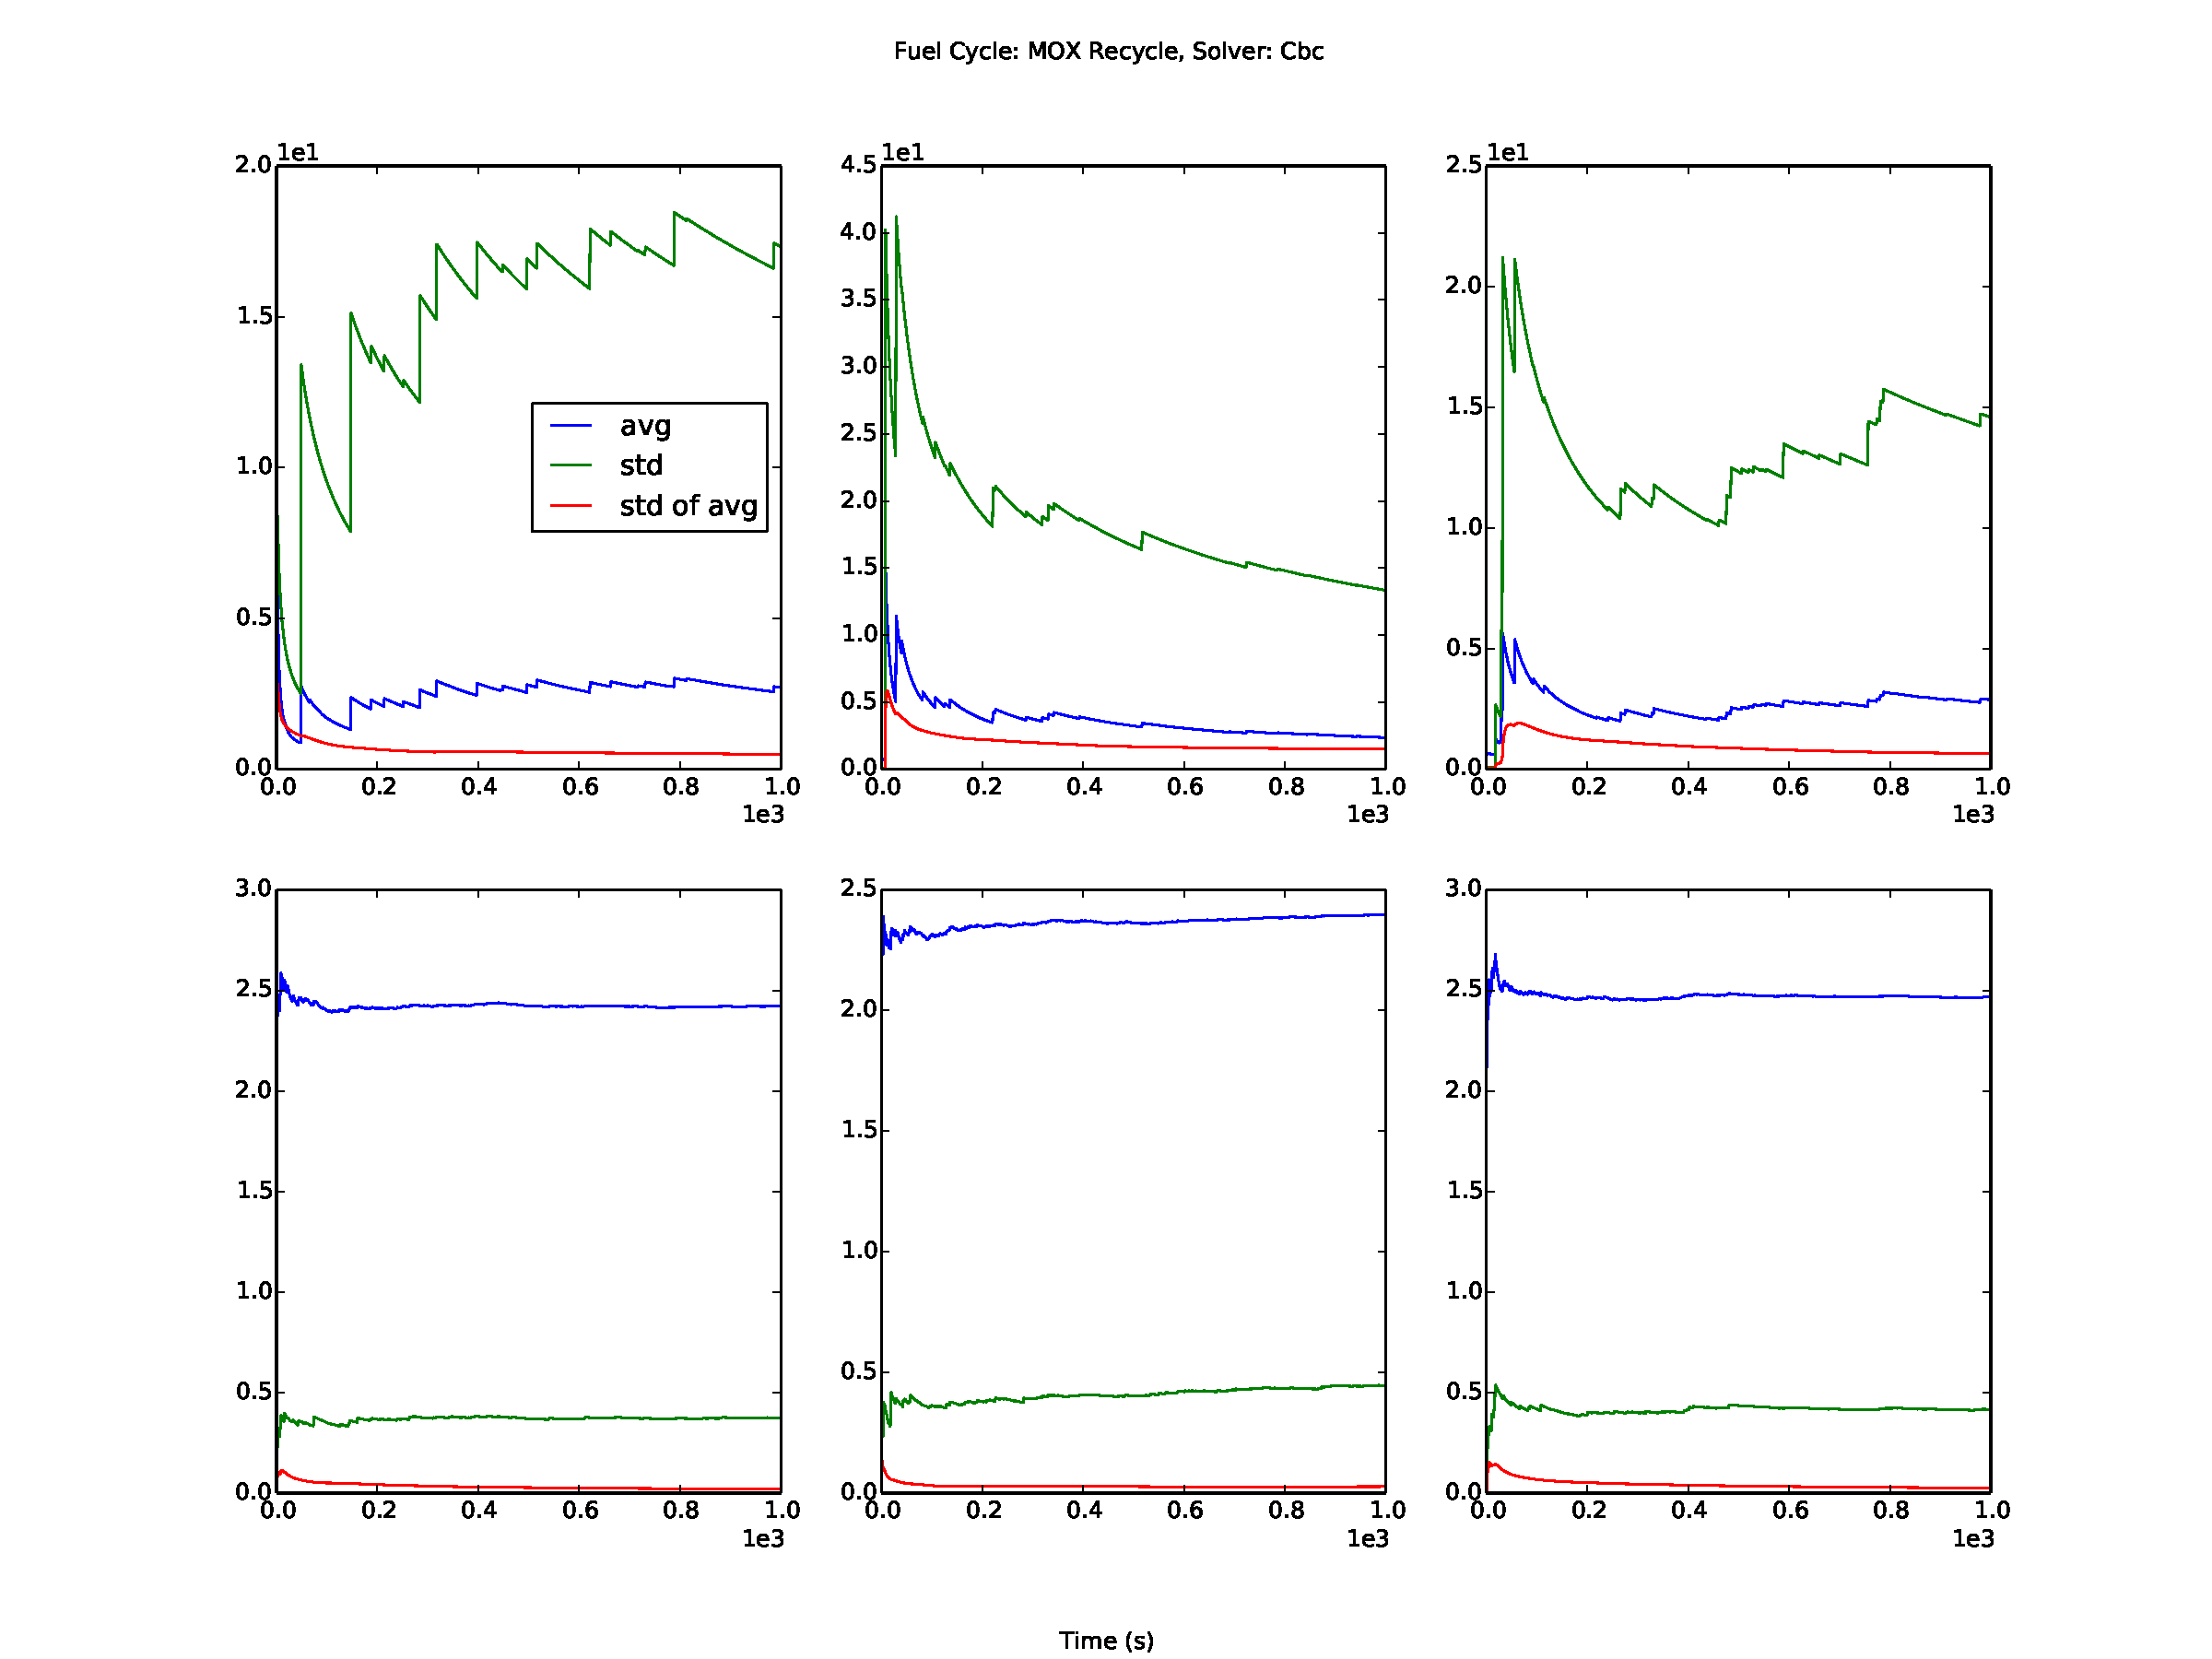
\includegraphics[width=1.5\columnwidth]{1k_avg_front_time_fc1_solvercbc.pdf}
    \caption[]{
      \label{fig:cbc_stochastic}
      Timing results for the stochastic study for the CBC Solver modeling a
      front-end MOX fuel cycle with $65$ reactors. Rows have increasing \frx
      values and columns have increasing \floc values.  }
  \end{center}
\end{figure*}

As can be seen in Figure \ref{fig:cbc_stochastic}, the CBC solver is sporadic
even for relatively small exchange sizes: some instances are solved very
quickly, while others can occasionally take a full allotted time before
returning. Interestingly, this behavior was seen much more frequently in
batch-based exchanges rather than assembly-based exchanges, likely due a more
constrained feasible solution space. Stochastic effects were also observed in
the solution times for the greedy heuristic and CLP solvers. However, average
solution times were found to converge after \textasciitilde$100$-$200$ instances
for both species of exchanges and all combinations of fundamental parameters.


%%%%%%%%%%%%%%%%%%%%%%%%%%%%%%%%%%%%%%%%%%%%%%%%%%%%%%%%%%%%%%%%%%%%%%%%%%%%%%%%
\section{Conclusions}

A first-of-a-kind analysis of the dynamic solution of supply and demand in a
nuclear fuel cycle is presented. A large number of exchanges are generated and
solved with a \Cyclus-aware greedy heuristic, the CLP solver, and the CBC
solver. The greedy heuristic is shown to scale well for very large problem
sizes, even when modeling up to $500$ reactors (on the order of the current
world-wide reactor population) trading individual assemblies. The CLP solver
also performs well at large problem scales. The CBC solver, while achieving the
true optimal solution in many cases, performs sporadically. Such a result is not
surprising, especially for highly-constrained optimization problems. Its use,
therefore, is suggested for initial exploratory studies before embarking on
full-fledged analytic campaigns. Most users will likely find the greedy
heuristic to be acceptable, as it provides a feasible solution and enables the
powerful features of the DRE.


%%%%%%%%%%%%%%%%%%%%%%%%%%%%%%%%%%%%%%%%%%%%%%%%%%%%%%%%%%%%%%%%%%%%%%%%%%%%%%%%
\section{Acknowledgments}

This research is being performed using funding received from the DOE
Office of Nuclear Energy's Nuclear Energy University Programs.  The
authors thank the NEUP for its generous support.

\begin{center}

\includegraphics[width=.25\columnwidth]{neup_logo_large.jpg}
\end{center}

The authors would like to especially thank Dr. Anthony M. Scopatz, whose advice
contributed greatly in the development of Cyclopts.

%%%%%%%%%%%%%%%%%%%%%%%%%%%%%%%%%%%%%%%%%%%%%%%%%%%%%%%%%%%%%%%%%%%%%%%%%%%%%%%%
\bibliographystyle{ans}
\bibliography{bibliography}
\end{document}
